\maketitle
\thispagestyle{fancy}

\begin{lefttextpipe}
	{\huge PŘEDSTAVENÍ SPOLEČNOSTI Proxy, a.s.}
\end{lefttextpipe}

Předmětem podnikání společnosti je především \textit{daňové poradenství} a \textit{činnost účetních poradců, vedení účetnictví, vedení daňové evidence}. Společnost má okolo 60 zaměstnanců\footnote{V Merku je možné dohledat číslo 50 - 99 zaměstnanců.}\textsuperscript{, }\footfullcite{noauthor_proxy_nodate} a je lokalizována v České republice. Společnost je součástí většího holdingu PROXY Holding a.s.. Společnost je dělená na několik oddělení, z nichž každá se soustředí na specifickou oblast v rámci daňového a účetního poradentsví, každá z těchto oblastní má vlastního manažera. Obecné směřování společnosti je stanovováno představenstvem.\\

Společnost se pohybuje výhradně na českém trhu v oblastni daňové a účetní, jejímy klienty jsou subjekty, které v České republice vykonávají jakoukoli ekonomickou činnost v rámci které jsou povinny řídit se českými daňovými a účetnímy předpisy. Hlavní službou společnost Proxy, a.s. je tak poskytování služeb související právě s činnostmi týkající se daní a vedení účetnictví a jedná se tedy výhradně o účetní a daňovou společnost.

\section*{A. Současná vize a poslání podniku}

\subsection*{A.1 Poslání a mise společnosti}

Dle informací na webových stránkách společnosti je základní poslání a mise poskytování služeb na poli daňového poradenství, účetnictví, mzdové evidence a dalšího specializovaného poradenství\footfullcite{noauthor_hlb_nodate}, především pro zahraniční investory vstupující na český trh a zjednodušit a zpřehlednit jim tam investici a fungování v České republice. 

\subsection*{A.2 Vize}

Vize společnosti spočívá především v tom, aby se stala partnerem pro své klienty a nadále je podporovala kvalifikovaným poradenstvím a to jak pro českou, tak i pro mezinárodní klientelu. Společnost se stala v roce 2004 součástí mezinárodní asociace poradenských firem HLB se sídlem v Londýně a nadále tak podporuje svojí vizi o kvalitní poradenské činnosti v dané oblasti.

\subsection*{A.3 Aktuální problémy}

S ohledem na informace na stránce a finanční výkazy (viz analýza níže) se společnost nepotýká s nedostatkem příležitostí a z nichž pramenícího zisku. Nejzásadnějším problémem je škálování vzhledem k dlouhodobému ekonomickému růstu a větší poptávce po daňovém a účetním poradenství, toto lze dovodit s ohledem jejich stránku kde chtějí studenty a mají permanentně vyvěšené pracovní nabídky, ČSÚ a vývoj počtu podnikatelů v dané oblastni a růstu vykazovanému v účetniství. Lze soudit ze statistik MPO odkaz za sledované období čtvrtého, respektive třetího kvartálu od roku 2016 až 2021

\begin{center}
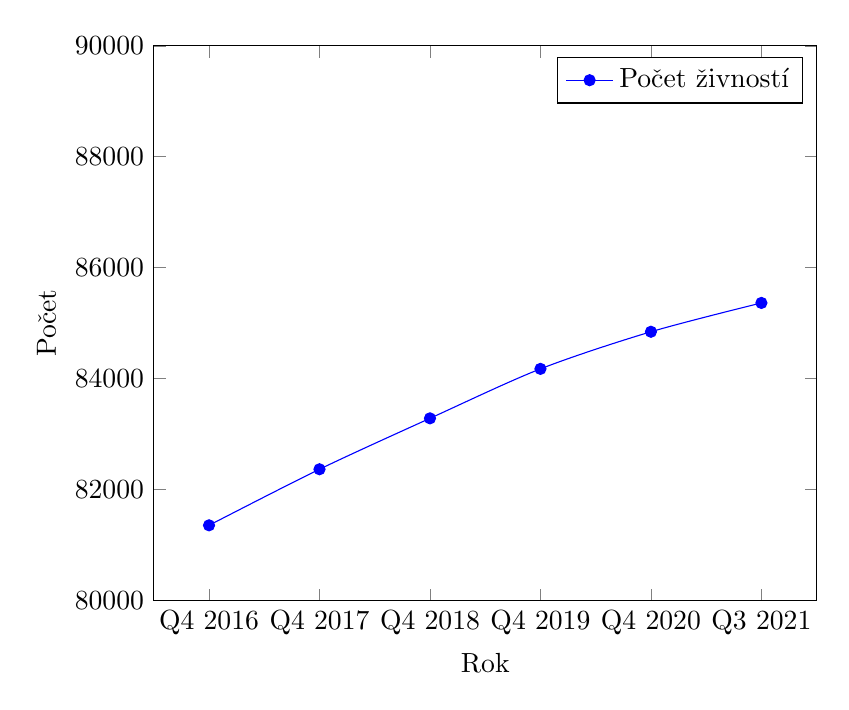
\begin{tikzpicture}
	\begin{axis}[
		width=10cm,
    	xlabel=Rok,
    	ylabel=Počet,
    	xmin=0, xmax=120,
    	ymin=80, ymax=90,
    	xtick={10,30,50,70,90,110},
    	xticklabels={Q4 2016,Q4 2017,Q4 2018,Q4 2019,Q4 2020,Q3 2021},   % <---
    	ytick={80,82,...,90},
    	yticklabels={80000, 82000, 84000, 86000, 88000, 90000}
            ]
		\addplot[smooth,mark=*,blue] 
			plot coordinates {
    			(10,81.354)
    			(30,82.365)
    			(50,83.283)
    			(70,84.175)
    			(90,84.844)
    			(110,85.364)
			};
		\addlegendentry{Počet živností}

	\end{axis}
\end{tikzpicture}
\end{center}

\newcommand\HorizontalSpaceBetweenNodes{2cm}

\begin{center}
\begin{tikzpicture}[node distance=2cm]
	
	% --- Starting node ---
	\node (start) [startstop] {SWOT / SFAS};
	
	% --- First left node ---
	\coordinate [below left of=start, node distance=2cm, xshift=-2cm] (update) {};
	\node (start1) [startstop, below left of=start, minimum width=6cm, xshift=-2cm, yshift=-2cm] {Vnější - PESTEL/STEEP (O+T)};
	
	% --- First right node ---
	\coordinate [below right of=start, node distance=2cm, xshift=2cm] (update2) {};
	\node (start2) [startstop, below right of=start, minimum width=6cm, xshift=2cm, yshift=-2cm] {Vnitřní (S+W)};
	
	% --- Second left nodes ---
	\coordinate [below left of=start1, node distance=2cm, xshift=-0.3cm] (update3) {};
	\node (start3) [startstop, below left of=start1, minimum width=2cm, xshift=-0.3cm, yshift=-2cm] {Odvětvové analýzy};
	\coordinate [below right of=start1, node distance=2cm, xshift=0.3cm] (update4) {};
	\node (start4) [startstop, below right of=start1, minimum width=2cm, xshift=0.3cm, yshift=-2cm] {Makro analýzy};
	
	
	% --- Second right nodes ---
	\coordinate [below left of=start2, node distance=2cm, xshift=-0.3cm] (update5) {};
	\node (start5) [startstop, below left of=start2, minimum width=2cm, xshift=-0.3cm, yshift=-2cm] {Zdroje a schopnosti};
	\coordinate [below right of=start2, node distance=2cm, xshift=0.3cm] (update6) {};
	\node (start6) [startstop, below right of=start2, minimum width=2cm, xshift=0.3cm, yshift=-2cm] {Podnik jako systém};
	
	% --- Third left nodes ---
	
	\node (start7) [startstop, below of=start3, minimum width=2.6cm] {Porter};
	\node (start8) [startstop, below of=start4, minimum width=2.6cm] {$u, \pi, FX, HDP$};
	
	% --- Third right nodes ---
	
	\node (start9) [startstop, below of=start5, minimum width=2.6cm] {VRIO};
	\node (start10) [startstop, below of=start6, minimum width=2.6cm, align=center] {Organizační\\(ne)efektivnost};
	
	\draw [arrow] (start) |- (update) -- (start1);
	\draw [arrow] (start) |- (update2) -- (start2);
	
	\draw [arrow] (start1) |- (update3) -- (start3);
	\draw [arrow] (start1) |- (update4) -- (start4);
	
	\draw [arrow] (start2) |- (update5) -- (start5);
	\draw [arrow] (start2) |- (update6) -- (start6);
	
	\draw [arrow] (start3) -- (start7);
	\draw [arrow] (start4) -- (start8);
	
	\draw [arrow] (start5) -- (start9);
	\draw [arrow] (start6) -- (start10);
	
\end{tikzpicture}
\end{center}


Taky bych sem měl zařadit analýzu, respektive graf rostoucích příjmů - pak rovněž odkázat na část, kde řeším příjmy v analýze.

Lze možná dooknce usoudit, že nárůst je způsobený i růstem příležitostí během COVIDU 19 a sním spojené nutnosti postarat se o daně a účetnivtví.


 a udržování knowledge basu a přizpůsobování procesů neustále se měnícím požadavkům na daňové a účetní, respektive finanční poradenství a povinnosti s ním související v českém právním prostoru, jedná se tedy o zásadní externí faktor.

\subsection*{A.4 Green deal}

Green deal je, odkaz, vztah společnosti ke green dealu je, blabla odkaz. Moc nemusí řešit green deal, nejsou výrobní společnost, která by generovala velké množství znečištění.

\section*{B. Identifikace procesu strategického řízení}

Úplně nemají, jenom základy podle kterých se řídí a jsou aktualizovány vedením společnosti, jsou v relativně stabilním businessu a pokrývají všechny oblasti v dané kategorii v četně auditu, takže úplně nepotřebují strategický plán.

Majá spíš operativní - na koho, kdy a jak se zaměří - maj i svojí klientelu, takže nepotřebují akvizici tak zásadně.

\section*{C. Popis současného obchodního modelu}

Současný model se soustředí na poskytování služeb v oblasti daňové a účetní a auditorské (v rámci jiné společnosti).

\newpage

\begin{table}[]
    \begin{tabular}{|l|lllll|}
        \hline
        \multicolumn{1}{|c|}{\multirow{2}{*}{\begin{tabular}[c]{@{}c@{}}Strategický ukazatel (které firma sleduje, případně\\ uveďte alespoň první tři)\end{tabular}}} & \multicolumn{5}{c|}{Vývoj v čase} \\ \cline{2-6} 
        \multicolumn{1}{|c|}{} & \multicolumn{1}{c|}{2016} & \multicolumn{1}{c|}{2017} & \multicolumn{1}{c|}{2018} & \multicolumn{1}{c|}{2019} & \multicolumn{1}{c|}{2020} \\ \hline
        Cash-flow celkem & \multicolumn{1}{l|}{} & \multicolumn{1}{l|}{} & \multicolumn{1}{l|}{} & \multicolumn{1}{l|}{} &  \\ \hline
        \begin{tabular}[c]{@{}l@{}}Investiční (kolik jde na rozvojové projekty a\\ aktiva, je zde záporné číslo? Dobře, investuje!)\end{tabular} & \multicolumn{1}{l|}{} & \multicolumn{1}{l|}{} & \multicolumn{1}{l|}{} & \multicolumn{1}{l|}{} &  \\ \hline
            Provozní (kolik příjmů má z hlavní činnosti) & \multicolumn{1}{l|}{} & \multicolumn{1}{l|}{} & \multicolumn{1}{l|}{} & \multicolumn{1}{l|}{} &  \\ \hline
            Finanční (výdaje na úvěry, finanční příjmy) & \multicolumn{1}{l|}{} & \multicolumn{1}{l|}{} & \multicolumn{1}{l|}{} & \multicolumn{1}{l|}{} &  \\ \hline
        \begin{tabular}[c]{@{}l@{}}Tržby z produkce vlastního zboží a služeb, popř. přidaná\\ hodnota, hrubá marže, cena, akcie.. a dlaší klíčové pro\\ firmu.\end{tabular} & \multicolumn{1}{l|}{} & \multicolumn{1}{l|}{} & \multicolumn{1}{l|}{} & \multicolumn{1}{l|}{} &  \\ \hline
    \end{tabular}
\caption{Test}
\label{tab:T}
\end{table}

\section*{D. Současné cíle společnosti}

\subsection*{D.1 Strategické}

Asi ovládnout trh.

\subsection*{D.2 Taktické}

Asi takticky ovládnout trh.

\section*{E. Odhad diskontních faktorů}

Haha test.

Test \footfullcite{noauthor_fideicommissum_nodate}

$EVA_t = NOPAT_t - WACC_t$ (aktiva celkem$_t -$ krátkodobé závazky$_t$)

\begin{table}[]
	\centering
	\makebox[\textwidth]{
		\begin{tabular}{llllll}
			\thickhline
			\multirow{2}{*}{} & \multicolumn{1}{c}{V} & \multicolumn{1}{c}{R} & \multicolumn{1}{c}{I} & \multicolumn{1}{c}{O} & \multicolumn{1}{c}{\multirow{2}{*}{Konkurenční výhoda}} \\
 				& \multicolumn{1}{c}{Hodnota?} & \multicolumn{1}{c}{Jedinečnost?} & \multicolumn{1}{c}{Nenapodob.?} & \multicolumn{1}{c}{Využito?} & \multicolumn{1}{c}{} \\
 			\thickhline
			Značka & Ano & Ano & Ano & Ano & Trvale udržitelná \\
			Distribuční síť & Ano & Ano & Ano & Ne & Plně nevyužitá \\
			\hline
			Finanční zdroje & Ano & Ano & Ano & Ne & Plně nevyužitá \\
			Lidské zdroje Management & Ano & Ano & Spíše ano & Ne & Plně nevyužitá \\
			Know-how & Ano & Ano & Ne &  & Dočasná \\
			Internetový obchod & Ano & Ano & Ne &  & Dočasná \\
			Pobočky & Ano & Ano & Ne &  & Dočasná \\
			Serverové řešení & Ano & Ne &  &  & Konkurenční parita \\
			Administrativa & Ano &  &  &  & Konkurenční nevýhoda \\
			\thickhline
		\end{tabular}}
\end{table}